\documentclass[12pt]{article}
\usepackage[utf8]{inputenc}
\usepackage[T1]{fontenc}
\usepackage[spanish]{babel}
\usepackage{graphicx}
\usepackage{geometry}
\usepackage{titlesec}
\usepackage{setspace}
\usepackage{hyperref}
\usepackage{enumitem}
\usepackage{listings}
\usepackage{xcolor}
\usepackage{framed}

% Configuración esencial para listings la vaina que permite mostrar código 
\definecolor{codebg}{rgb}{0.95,0.95,0.95}
\lstset{
    backgroundcolor=\color{codebg},
    basicstyle=\ttfamily\footnotesize,
    breaklines=true,
    frame=single,
    language=SQL,
    numbers=left,
    numberstyle=\tiny\color{gray},
    captionpos=b
}

% Configuración de página
\geometry{letterpaper, margin=2.5cm}
\setlength{\parskip}{1em}
\setlength{\parindent}{0pt}
\titleformat{\section}{\centering\large\bfseries}{}{0em}{}
\titleformat{\subsection}{\centering\normalsize\bfseries}{}{0em}{}
\titleformat{\subsubsection}{\centering\small\bfseries}{}{0em}{}

% Configuración de hipervínculos
\hypersetup{
    colorlinks=true,
    linkcolor=blue,
    urlcolor=blue,
    pdftitle={Mini Plataforma de Video Streaming P2P con Microservicios},
    pdfauthor={Aaron Rodrigo Ramos Reyes, Oscar Martinez Barrales, Oswaldo Mejia Garcia}
}

\begin{document}

% Portada
\begin{titlepage}
    \centering
    \vspace*{3cm}
    {\Huge\bfseries Sistemas Distribuidos \par}
    \vspace{2cm}
    {\Large Mini Plataforma de Video Streaming P2P con Microservicios\par}
    \vspace{3cm}
    {\large Autores:\par}
    \vspace{0.5cm}
    {\normalsize Aaron Rodrigo Ramos Reyes\par}
    {\normalsize Oscar Martinez Barrales\par}
    {\normalsize Oswaldo Mejia Garcia\par}
    \vfill
    {\large Universidad Autonoma Metropolitana\par}
    {\large Fecha: \today\par}
\end{titlepage}

% Índice

\newpage

% Sección de introducción
\section*{Introducción}  

El presente proyecto consiste en la implementación de una \textbf{mini plataforma de video streaming P2P con microservicios}, cuyo objetivo es permitir que diferentes nodos intercambien fragmentos de video de manera distribuida, sin depender de un único servidor central para el envío de datos.

\subsection*{Planteamiento del Problema}
Las plataformas de streaming tradicionales dependen de un servidor central que entrega el contenido directamente a cada usuario. Esto genera un cuello de botella cuando muchos usuarios solicitan el mismo video.  
En este proyecto se busca aprovechar el \textbf{modelo P2P} para que cada nodo no solo consuma, sino que también comparta fragmentos con otros, reduciendo la carga central.

\subsection*{Estructura de la Solución}
La solución se basa en tres elementos clave:
\begin{enumerate}
    \item \textbf{Servicio Central (Registry Service)}: Registra nodos y mantiene un mapeo de qué fragmentos posee cada uno.
    \item \textbf{Nodos P2P}: Almacenan y comparten fragmentos de video, comunicándose directamente para transferir datos.
    \item \textbf{Sistema Pub/Sub con Redis}: Notifica a los nodos cuando hay nuevos fragmentos disponibles.
\end{enumerate}

\subsection*{Diagrama de Arquitectura}
Diseño del esquema general del sistema, incluyendo el servicio central, los nodos P2P y el canal de comunicación Pub/Sub.

\begin{center}
    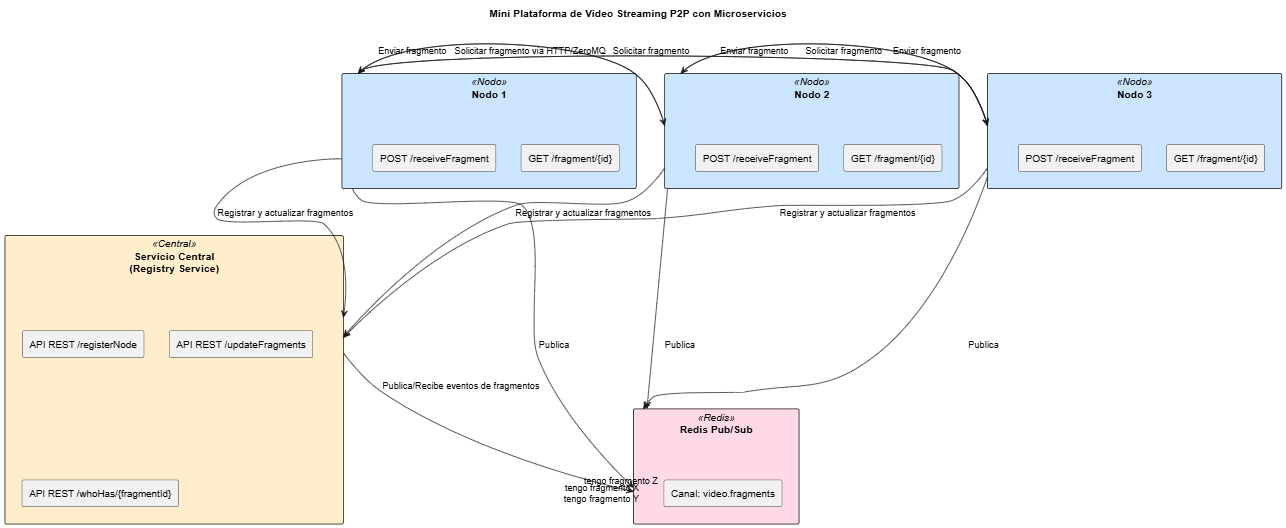
\includegraphics[width=\textwidth]{Diagramas/Diagrama.png}
\end{center}


% Arquitectura del Sistema
\section*{Arquitectura del Sistema}
La arquitectura del sistema se basa en un modelo híbrido que combina elementos centralizados y distribuidos para optimizar la distribución de contenido de video.

\subsection*{Componentes Principales}

\subsubsection*{Servicio Central (Registry Service)}
El servicio central actúa como un registro y coordinador del sistema, implementado como un microservicio Spring Boot que:

\begin{itemize}
    \item Mantiene un registro de todos los nodos activos en la red
    \item Almacena información sobre qué fragmentos posee cada nodo
    \item Proporciona APIs REST para consultas de ubicación de fragmentos
    \item Gestiona el sistema de notificaciones Pub/Sub con Redis
\end{itemize}

\textbf{Endpoints principales:}
\begin{itemize}
    \item \texttt{POST /api/register} - Registro de nuevos nodos
    \item \texttt{GET /api/nodes} - Lista de nodos registrados
    \item \texttt{GET /api/fragment/\{fragmentId\}} - Localización de fragmentos
    \item \texttt{POST /api/updateFragments} - Actualización de inventario de fragmentos
\end{itemize}

\subsubsection*{Nodos P2P}
Cada nodo P2P es un microservicio independiente que:

\begin{itemize}
    \item Almacena fragmentos de video localmente
    \item Sirve fragmentos a otros nodos mediante HTTP
    \item Se registra automáticamente en el servicio central al iniciar
    \item Escucha notificaciones de nuevos fragmentos disponibles
    \item Implementa lógica de descarga automática de fragmentos faltantes
\end{itemize}

\textbf{Endpoints principales:}
\begin{itemize}
    \item \texttt{GET /fragment/\{id\}} - Descarga de fragmentos
    \item \texttt{POST /fragment/receive} - Recepción de fragmentos
\end{itemize}

\subsubsection*{Sistema Pub/Sub con Redis}
Redis actúa como broker de mensajes para:

\begin{itemize}
    \item Notificar a todos los nodos cuando hay nuevos fragmentos disponibles
    \item Mantener la sincronización del estado del sistema
    \item Reducir la carga en el servicio central mediante notificaciones asíncronas
\end{itemize}

\subsection*{Flujo de Comunicación}

\begin{enumerate}
    \item Los nodos se registran en el servicio central al iniciar
    \item Cuando un nodo recibe un nuevo fragmento, notifica al servicio central
    \item El servicio central publica un evento en Redis
    \item Otros nodos reciben la notificación y pueden solicitar el fragmento
    \item La transferencia de fragmentos ocurre directamente entre nodos (P2P)
\end{enumerate}

\subsection*{Escalabilidad y Tolerancia a Fallos}

El sistema está diseñado para escalar horizontalmente:

\begin{itemize}
    \item Nuevos nodos pueden unirse dinámicamente
    \item La carga se distribuye automáticamente entre nodos
    \item Si un nodo falla, otros nodos pueden tener copias de sus fragmentos
    \item El servicio central puede replicarse para alta disponibilidad
\end{itemize}

% Implementación
\section*{Implementación}
\subsection*{Estructura del Proyecto}

El proyecto está organizado en dos microservicios principales:

\begin{itemize}
    \item \textbf{centralservice} - Servicio de registro y coordinación
    \item \textbf{p2pnodo} - Nodos P2P para almacenamiento y distribución
\end{itemize}
\newpage
\subsection*{Servicio Central}

\subsubsection*{Modelos de Datos}

\textbf{NodeRegistration.java}
\begin{lstlisting}[language=Java]
public class NodeRegistration {
    private String nodeId;
    private String nodeUrl;
    private List<String> fragments;
    // getters y setters
}
\end{lstlisting}

\textbf{FragmentEvent.java}
\begin{lstlisting}[language=Java]
public class FragmentEvent {
    private String fragmentId;
    private String nodeUrl;
    private Long timestamp;
    
    public boolean isValid() {
        return fragmentId != null && !fragmentId.isEmpty() &&
               nodeUrl != null && !nodeUrl.isEmpty();
    }
}
\end{lstlisting}

\subsubsection*{Controladores REST}

El servicio central expone endpoints REST para:
\begin{itemize}
    \item Registro de nodos
    \item Consulta de nodos disponibles
    \item Localización de fragmentos específicos
    \item Actualización de inventarios de fragmentos
\end{itemize}

\subsection*{Nodos P2P}

\subsubsection*{Auto-registro}

Cada nodo se registra automáticamente al iniciar usando \texttt{@PostConstruct}:

\begin{lstlisting}[language=Java]
@PostConstruct
public void registerOnStartup() {
    NodeRegistration registration = new NodeRegistration();
    registration.setNodeId(System.getenv("HOSTNAME"));
    registration.setNodeUrl(NODE_URL);
    registration.setFragments(List.of());
    
    restTemplate.postForObject(
        CENTRAL_SERVICE_URL + "/api/register",
        registration,
        String.class
    );
}
\end{lstlisting}

\subsubsection*{Cliente de Comunicación P2P}

La clase \texttt{NodeClient} maneja la comunicación entre nodos:

\begin{itemize}
    \item \textbf{downloadFragment()} - Descarga fragmentos de otros nodos
    \item \textbf{uploadFragment()} - Envía fragmentos usando multipart/form-data
\end{itemize}

\subsection*{Gestión de Fragmentos}

Los fragmentos se almacenan como archivos binarios y se transfieren usando:
\begin{itemize}
    \item HTTP multipart para subida de archivos
    \item Streaming de bytes para descarga
    \item Validación de integridad mediante IDs únicos
\end{itemize}

\subsection*{Configuración con Docker}

El sistema utiliza Docker Compose para orquestación:

\begin{itemize}
    \item \textbf{Redis} - Base de datos y Pub/Sub
    \item \textbf{Central Service} - Un contenedor
    \item \textbf{P2P Nodes} - Múltiples contenedores escalables
\end{itemize}

\textbf{Comando de despliegue:}
\begin{lstlisting}[language=bash]
docker compose up -d --scale p2pnodo=3
\end{lstlisting}

\subsection*{Manejo de Errores y Logging}

El sistema implementa:
\begin{itemize}
    \item Manejo de excepciones en comunicaciones HTTP
    \item Validación de datos de entrada
    \item Timeouts configurables para operaciones de red
\end{itemize}

% Tecnologías Utilizadas
\section*{Tecnologías Utilizadas}
\subsection*{Backend}

\subsubsection*{Java}
Lenguaje de programación principal del proyecto, aprovechando las características más recientes como:
\begin{itemize}
    \item Records para DTOs inmutables
    \item Mejor rendimiento y gestión de memoria
\end{itemize}

\subsubsection*{Spring Boot}
Framework principal para el desarrollo de microservicios:
\begin{itemize}
    \item \textbf{Spring Web} - APIs REST
    \item \textbf{Spring Data Redis} - Integración con Redis
    \item \textbf{Spring Boot Actuator} - Monitoreo y métricas
\end{itemize}

\subsubsection*{Maven}
Herramienta de gestión de dependencias y construcción:
\begin{itemize}
    \item Gestión automática de dependencias
    \item Perfiles de construcción para diferentes entornos
    \item Plugins para empaquetado Docker
\end{itemize}

\subsection*{Base de Datos y Mensajería}

\subsubsection*{Redis}
Sistema de almacenamiento en memoria que proporciona:
\begin{itemize}
    \item \textbf{Pub/Sub} - Sistema de mensajería para notificaciones
    \item \textbf{Cache} - Almacenamiento rápido de metadatos
    \item \textbf{Persistencia} - Respaldo de datos críticos
\end{itemize}

\subsection*{Herramientas de Desarrollo}


\subsubsection*{Swagger}
Documentación automática de APIs:
\begin{itemize}
    \item Generación automática de documentación
    \item Interfaz web interactiva para pruebas
\end{itemize}

\subsubsection*{Jackson}
Serialización/deserialización JSON:
\begin{itemize}
    \item Conversión automática de objetos Java a JSON
    \item Configuración flexible de mapeo
    \item Soporte para tipos complejos
\end{itemize}

\subsection*{Containerización y Orquestación}

\subsubsection*{Docker}
Containerización de aplicaciones:
\begin{itemize}
    \item Imágenes ligeras basadas en OpenJDK
    \item Configuración mediante variables de entorno
    \item Aislamiento de dependencias
\end{itemize}

\subsubsection*{Docker Compose}
Orquestación de múltiples servicios:
\begin{itemize}
    \item Definición declarativa de servicios
    \item Escalado horizontal automático
    \item Gestión de redes y volúmenes
\end{itemize}


% Calendario de Actividades
\section*{Calendario de Actividades}
\subsection*{Cronograma del Proyecto}

El proyecto se desarrolló en un período intensivo de 5 días (4-8 de agosto de 2025), con una distribución equitativa de responsabilidades entre los tres integrantes del equipo.

\subsection*{Distribución de Actividades por Día}

\subsubsection*{Lunes 4 de Agosto - Planificación y Diseño}

\textbf{Aaron Rodrigo Ramos Reyes:}
\begin{itemize}
    \item Análisis de requisitos del sistema P2P
    \item Diseño de la arquitectura general del sistema
    \item Definición de APIs REST para el servicio central
    \item Creación de diagramas de arquitectura (PlantUML)
\end{itemize}

\textbf{Oscar Martinez Barrales:}
\begin{itemize}
    \item Investigación de tecnologías P2P y microservicios
    \item Diseño de la estructura de datos para fragmentos
    \item Definición de protocolos de comunicación entre nodos
    \item Configuración inicial del entorno de desarrollo
\end{itemize}

\textbf{Oswaldo Mejia Garcia:}
\begin{itemize}
    \item Análisis de patrones de distribución de contenido
    \item Diseño del sistema Pub/Sub con Redis
    \item Configuración de Docker y Docker Compose
\end{itemize}

\subsubsection*{Martes 5 de Agosto - Desarrollo del Servicio Central}

\textbf{Aaron Rodrigo Ramos Reyes:}
\begin{itemize}
    \item Implementación del servicio central (Spring Boot)
    \item Desarrollo de controladores REST
    \item Configuración de Spring Data Redis
    \item Implementación de DTOs (NodeRegistration, FragmentEvent)
\end{itemize}

\textbf{Oscar Martinez Barrales:}
\begin{itemize}
    \item Desarrollo de la lógica de registro de nodos
    \item Implementación del sistema de localización de fragmentos
    \item Configuración de validaciones con Hibernate Validator
    \item Desarrollo de servicios de negocio
\end{itemize}

\textbf{Oswaldo Mejia Garcia:}
\begin{itemize}
    \item Configuración de Redis Pub/Sub
    \item Implementación de listeners de eventos
    \item Desarrollo de la lógica de notificaciones
\end{itemize}

\subsubsection*{Miércoles 6 de Agosto - Desarrollo de Nodos P2P}

\textbf{Aaron Rodrigo Ramos Reyes:}
\begin{itemize}
    \item Implementación de la aplicación P2P Node
    \item Desarrollo de controladores para fragmentos
    \item Implementación de auto-registro en el servicio central

\end{itemize}

\textbf{Oscar Martinez Barrales:}
\begin{itemize}
    \item Desarrollo de NodeClient para comunicación P2P
    \item Implementación de descarga de fragmentos
    \item Configuración de RestTemplate para comunicación HTTP
\end{itemize}

\textbf{Oswaldo Mejia Garcia:}
\begin{itemize}
    \item Implementación de almacenamiento local de fragmentos
    \item Desarrollo de la lógica de sincronización
    \item Configuración de variables de entorno
\end{itemize}

\subsubsection*{Jueves 7 de Agosto - Integración y Testing}

\textbf{Aaron Rodrigo Ramos Reyes:}
\begin{itemize}
    \item Integración completa del sistema
    \item Configuración de Docker Compose
\end{itemize}

\textbf{Oscar Martinez Barrales:}
\begin{itemize}
    \item Testing de APIs con Postman
    \item Validación de transferencia de fragmentos
\end{itemize}

\textbf{Oswaldo Mejia Garcia:}
\begin{itemize}
    \item Validación de notificaciones en tiempo real
    \item Testing de tolerancia a fallos
\end{itemize}

\subsubsection*{Viernes 8 de Agosto - Documentación y Entrega}

\textbf{Aaron Rodrigo Ramos Reyes:}
\begin{itemize}
    \item Redacción de documentación técnica
    \item Creación de instructivos de instalación
    \item Preparación de la presentación final
    \item Revisión final del código
\end{itemize}

\textbf{Oscar Martinez Barrales:}
\begin{itemize}
    \item Documentación de APIs con OpenAPI/Swagger
    \item Creación de guías de uso con Postman
    \item Documentación de arquitectura
    \item Testing final del sistema completo
\end{itemize}

\textbf{Oswaldo Mejia Garcia:}
\begin{itemize}
    \item Documentación de despliegue con Docker
    \item Creación de scripts de automatización
    \item Documentación de configuración
    \item Preparación de entregables finales
\end{itemize}

\subsection*{Metodología de Trabajo}

\begin{itemize}
    \item \textbf{Control de versiones:} Git con ramas por funcionalidad
    \item \textbf{Comunicación:} Discord para coordinación continua
    \item \textbf{Testing continuo:} Validación diaria de integraciones
\end{itemize}



% Conclusiones
\section*{Conclusiones}


El proyecto de Mini Plataforma de Video Streaming P2P con Microservicios ha cumplido exitosamente con todos los objetivos planteados:

\begin{itemize}
    \item \textbf{Arquitectura Distribuida:} Se implementó un sistema híbrido que combina un servicio central de registro con comunicación P2P directa entre nodos
    \item \textbf{Escalabilidad:} El sistema permite agregar nodos dinámicamente usando Docker Compose con escalado horizontal
    \item \textbf{Comunicación Eficiente:} Se estableció un sistema de notificaciones en tiempo real usando Redis Pub/Sub
    \item \textbf{Transferencia de Fragmentos:} Los nodos pueden intercambiar fragmentos de video de manera directa y eficiente
\end{itemize}

\subsection*{Beneficios del Enfoque P2P}

La implementación P2P demostró ventajas significativas sobre modelos centralizados tradicionales:

\begin{itemize}
    \item \textbf{Reducción de Carga Central:} El servidor central solo maneja registro y coordinación, no transferencia de datos
    \item \textbf{Tolerancia a Fallos:} Los fragmentos pueden estar replicados en múltiples nodos
    \item \textbf{Escalabilidad Natural:} Más nodos significan más capacidad total del sistema
\end{itemize}


\subsubsection*{Microservicios con Spring Boot}
La arquitectura de microservicios permitió:
\begin{itemize}
    \item Desarrollo independiente de componentes
    \item Mantenimiento simplificado
\end{itemize}

\subsubsection*{Containerización con Docker}
El uso de Docker facilitó:
\begin{itemize}
    \item Despliegue consistente en diferentes entornos
    \item Escalado automático de nodos
    \item Aislamiento de dependencias
    \item Configuración simplificada
\end{itemize}

\subsubsection*{Sistema Pub/Sub}
Redis Pub/Sub proporcionó:
\begin{itemize}
    \item Notificaciones en tiempo real
    \item Desacoplamiento entre componentes
    \item Sincronización de estado distribuido
\end{itemize}

\subsection*{Desafíos Superados}

Durante el desarrollo se enfrentaron y resolvieron varios desafíos técnicos:

\begin{itemize}
    \item \textbf{Sincronización de Estado:} Implementación de un sistema robusto de notificaciones para mantener consistencia
    \item \textbf{Transferencia de Archivos:} Desarrollo de un mecanismo eficiente para transferir fragmentos entre nodos
    \item \textbf{Auto-registro:} Configuración automática de nodos al iniciar usando variables de entorno
    \item \textbf{Manejo de Errores:} Implementación de tolerancia a fallos en comunicaciones de red
\end{itemize}



Este proyecto proporcionó experiencia práctica en:

\begin{itemize}
    \item Desarrollo de sistemas distribuidos
    \item Arquitectura de microservicios
    \item Comunicación P2P
    \item Containerización y orquestación
    \item Trabajo colaborativo en equipo
    \item Metodologías ágiles de desarrollo
\end{itemize}




\end{document}